

%%% Uncomment for slide version
\documentclass{beamer}
\setbeameroption{hide notes} % Only slides

%%% Uncomment for handout version
%\documentclass[handout]{beamer}
%\setbeameroption{show notes on second screen=right} % Both

\setbeamertemplate{note page}{\pagecolor{white}\insertnote}

\setbeamertemplate{footline}{}

\usetheme[progressbar=frametitle]{moloch}% modern fork of the metropolis theme

\setbeamercolor{background canvas}{bg=white}
\setbeamercolor{progress bar}{use=palette primary,fg=red,bg=red}

\setbeamercolor{note page}{bg=white} 

\setbeamertemplate{date}{}


\defbeamertemplate*{title page}{customized}[1][]
{
	\usebeamerfont{title}\inserttitle\par
	\bigskip
	\bigskip
		\bigskip
			\bigskip

	\usebeamerfont{title}\usebeamercolor[fg]{subtitle}\insertsubtitle\par
	\bigskip
	\usebeamerfont{author}\insertauthor\par
	\usebeamerfont{subtitle}\insertinstitute\par
	\usebeamercolor[fg]{titlegraphic}\inserttitlegraphic
}

\addtobeamertemplate{navigation symbols}{}{%
	\usebeamerfont{footline}%
	\usebeamercolor[fg]{footline}%
	\hspace{1em}%
	\insertframenumber/\inserttotalframenumber
}
\setbeamercolor{itemize item}{fg=black}
\setbeamercolor{itemize subitem}{fg=black}
\setbeamercolor{itemize subsubitem}{fg=black}

%%% Slide 1

\title{\Huge FRST302: Forest Genetics}
\author{\Large Lecture 1.1: Classical Genetics and its Molecular Mechanisms}
\date{\today}

\begin{document}
	\maketitle

\note{\emph{Remember, everything on the lecture slides and the accompanying notes is potentially examinable!}}
% for the beamer version
%\documentclass{beamer}


%%% Slide 3
	
\begin{frame}
		\frametitle{Outline for Today}
\setbeamertemplate{itemize items}[circle]
\Large{
			\begin{itemize} 
			\item Short history of genetics
			\item Mendel's laws
			\item Chromosomes
		\end{itemize}
	}

\note{
Learning Outcomes
	\emph{		\begin{itemize} 
				\item Basic definitions in genetics
				\item Principles and terms in classical genetics
				\item Molecular mechanisms of classical genetics
				\item Chromosome crossover and its significance
			\end{itemize}
	}
}
\end{frame}

%%% Slide 4
\begin{frame}
\frametitle{History of Genetics}

\Large \textbf{What is genetics?} \par

\bigskip
\pause
\Large \textbf{Genetics is the study of genes}, of variation and heredity across all branches of the tree of life




\end{frame}



%%% Slide 2

\begin{frame}
	
	\Huge \centering \emph{What are the major questions in genetics?}
	\vspace{20pt}
	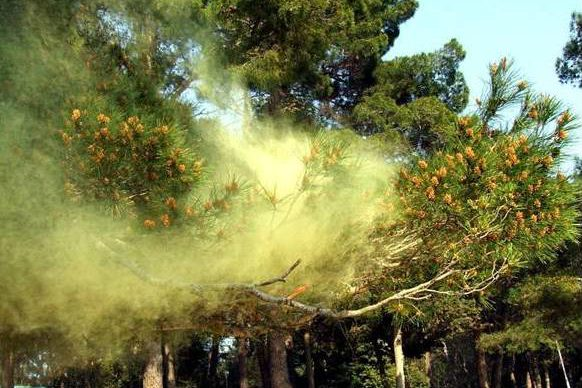
\includegraphics[keepaspectratio, width  =0.8\textwidth]{img/pollenPlume}
	\note{
		The answer to this question totally depends on your perspective. However, I think that it is more than fair to say that the following questions are at the heart of most biological science:
		\begin{itemize} 
			\item Why is there so much variation among individuals?
			\item How is this variation maintained in populations?
			\item Why do offspring tend to resemble their parents? 
			\par
		\end{itemize}
		
		\footnote \url{https://www.asthmacenter.com/wp-content/uploads/Pine-Pollen-Plume-e1495119706845.jpg}
	}
\end{frame}


\begin{frame}
	
	How can we apply a knowledge of genetics?
	
	\vspace{5pt}
	
	\centering
	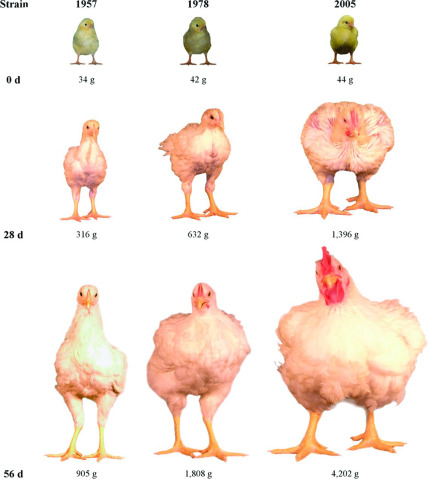
\includegraphics[keepaspectratio, width  =0.6\textwidth]{img/zuidhof_2014} \footnote {Modified from Figure 1 - Zuidhof et al. 2014}
\end{frame}

\begin{frame}
	\frametitle{History of Genetics}
	
\begin{columns}[T]
	\begin{column}{.7\textwidth}
			Humans have probably pondered inheritence for all history:
			\vspace{10pt}
			\begin{itemize}
				\item For much of history, the mechanisms of inheritence were basically unknown
				\item The inheritance of acquired characteristics was widely accepted for much of history (from Hippocrates to Aristotal to Lamarck) \pause
				\item \emph{Early microscopists thought that they had seen small humans inhabiting sperm cells!}
			\end{itemize}
	\end{column}
	\begin{column}{.3\textwidth}
			% Your image included here
% TODO: \usepackage{graphicx} required
\centering
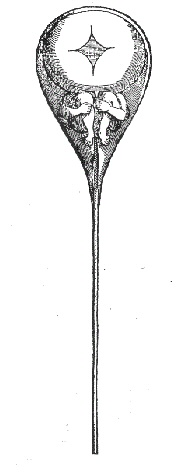
\includegraphics[keepaspectratio, width  = 0.8\textwidth]{img/homunculous}\footnotemark[1]


	\end{column}
\end{columns}
   \note{
	The inheritance of acquired characteristics is often referred to simply as Lamarkism after Jean-Baptiste Lamarck.

	Lamarck was an 19th century evolutionary biologist who formalised a lot of the contemporary thought on how biodiversity originated. The classic example is a giraffe stretching up to reach higher leaves would likely give birth to offspring with longer necks.
	
	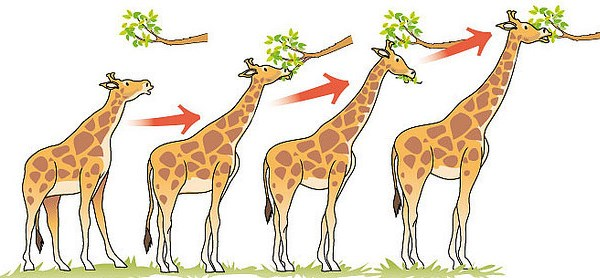
\includegraphics[keepaspectratio, width  = 0.8\textwidth]{img/lamarck}\\
			\url{https://simple.wikipedia.org/wiki/Lamarckism}
}
\end{frame}



\begin{frame}
	\frametitle{History of Genetics}
	
	\begin{columns}[T]
		\begin{column}{.6\textwidth}
			By the time Darwin came around, the dominant theory was \textbf{blending inheritance}
		
			\vspace{10pt}
			\begin{itemize}
				\item The notion that an offspring's traits are simply the average of the parents' traits. 
				\item This is intuitively appealing - offspring's traits are often intermediate 
				\item There is one big problem with blending inheritance!
			\end{itemize}
		\end{column}
		\begin{column}{.3\textwidth}
				\centering
			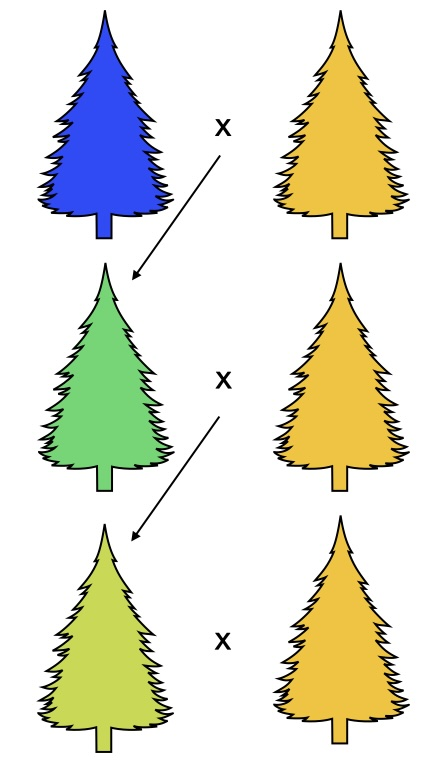
\includegraphics[keepaspectratio, width  = 1.1\textwidth]{img/blending}
		\end{column}
	\end{columns}
	

\end{frame}
	
\begin{frame}
		\frametitle{The Problem with Blending}
		
				\Huge \centering \emph{What's the big problem with blending inheritance?}
		   \note{The halving of variation each generation due to blending inheritance was first pointed out by Fleeming Jenkin - the inventor of the cable car}
\end{frame}





\end{document}